\section{Diseño del modelo elástico}
\subsection*{Análisis del modelo elástico}

\addtocounter{framenumber}{-1}
\begin{frame}[t]{Contenidos}{\textcolor{UniBlue}{.}}
	\tableofcontents[currentsection]
\end{frame}

\begin{frame}[t]{Diseño del modelo elástico}{Análisis del modelo elástico}
\begin{itemize}
\item Recursos lógicos del sistema según el enfoque dinámico
\item Bajo overhead $\rightarrow$ Escalable
\item Técnica de fisión
\begin{itemize}
	\item Elasticidad $\rightarrow$ Añadir/Reducir la cantidad de réplicas del operador
	\item Solucionando:
	\begin{itemize}
		\item Sobrecarga
		\item Utilización de recursos
	\end{itemize}
\end{itemize}
\end{itemize}

\begin{picture}(0,150)
	\put(90,75){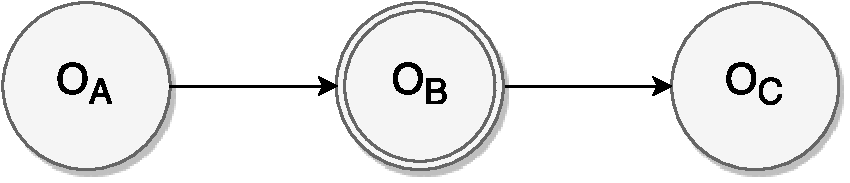
\includegraphics[scale=.35]{images/EjReplicacion-I.pdf}}
\end{picture}

\end{frame}

\addtocounter{framenumber}{-1}
\begin{frame}[t]{Diseño del modelo elástico}{Análisis del modelo elástico}
\begin{itemize}
\item Recursos lógicos del sistema según el enfoque dinámico
\item Bajo overhead $\rightarrow$ Escalable
\item Técnica de fisión
\begin{itemize}
	\item Elasticidad $\rightarrow$ Añadir/Reducir la cantidad de réplicas del operador
	\item Solucionando:
	\begin{itemize}
		\item Sobrecarga
		\item Utilización de recursos
	\end{itemize}
\end{itemize}
\end{itemize}

\begin{picture}(0,150)
	\put(90,55){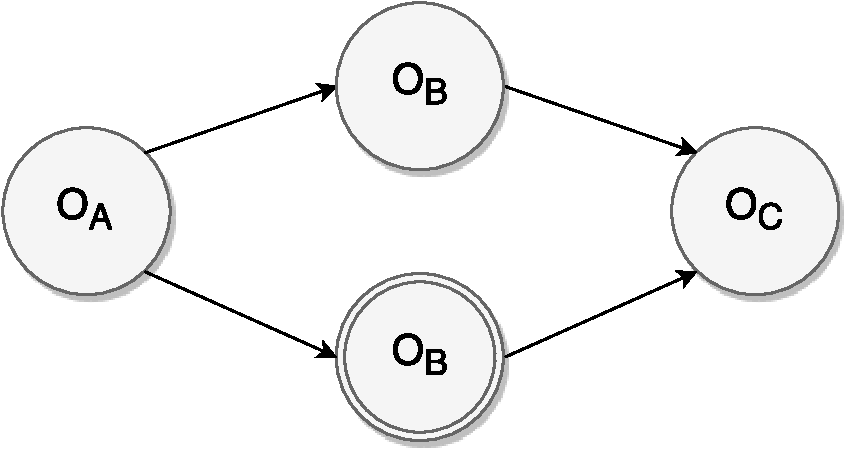
\includegraphics[scale=.35]{images/EjReplicacion-II.pdf}}
\end{picture}

\end{frame}

\addtocounter{framenumber}{-1}
\begin{frame}[t]{Diseño del modelo elástico}{Análisis del modelo elástico}
\begin{itemize}
\item Recursos lógicos del sistema según el enfoque dinámico
\item Bajo overhead $\rightarrow$ Escalable
\item Técnica de fisión
\begin{itemize}
	\item Elasticidad $\rightarrow$ Añadir/Reducir la cantidad de réplicas del operador
	\item Solucionando:
	\begin{itemize}
		\item Sobrecarga
		\item Utilización de recursos
	\end{itemize}
\end{itemize}
\end{itemize}

\begin{picture}(0,150)
	\put(90,35){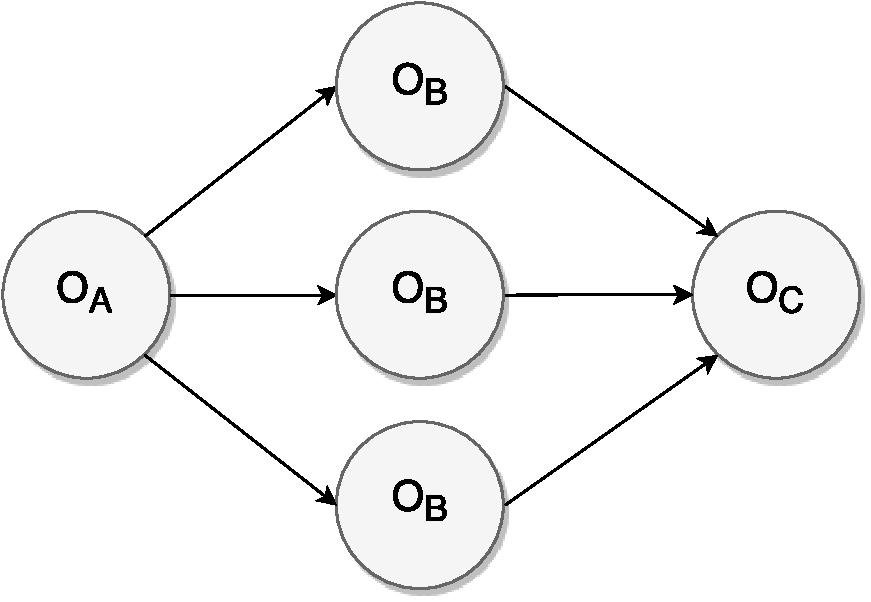
\includegraphics[scale=.35]{images/EjReplicacion-III.pdf}}
\end{picture}

\end{frame}

\begin{frame}{Diseño del modelo elástico}{Análisis del modelo elástico}
\begin{itemize}
\item El modelo elástico está basado en la teoría de colas
\begin{itemize}
	\item Tasa de rendimiento $\rho$
	\item $\rho = \frac{\lambda}{s \mu}$
\end{itemize}	
\end{itemize}

\begin{figure}[!hb]
	\centering
	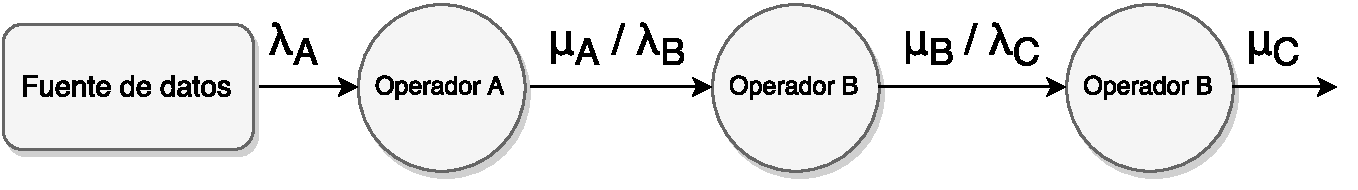
\includegraphics[scale=0.45]{images/AnalisisTeoriaColas.pdf}
\end{figure}

\end{frame}

\begin{frame}{Diseño del modelo elástico}{Análisis del modelo elástico}
\begin{itemize}
	\item Se propone un modelo elástico compuesto por 4 módulos
	\item Basado en el modelo MAPE (Monitoreo, Análisis, Procesamiento y Ejecución)
\end{itemize}
\begin{figure}[ht!]
  \centering
    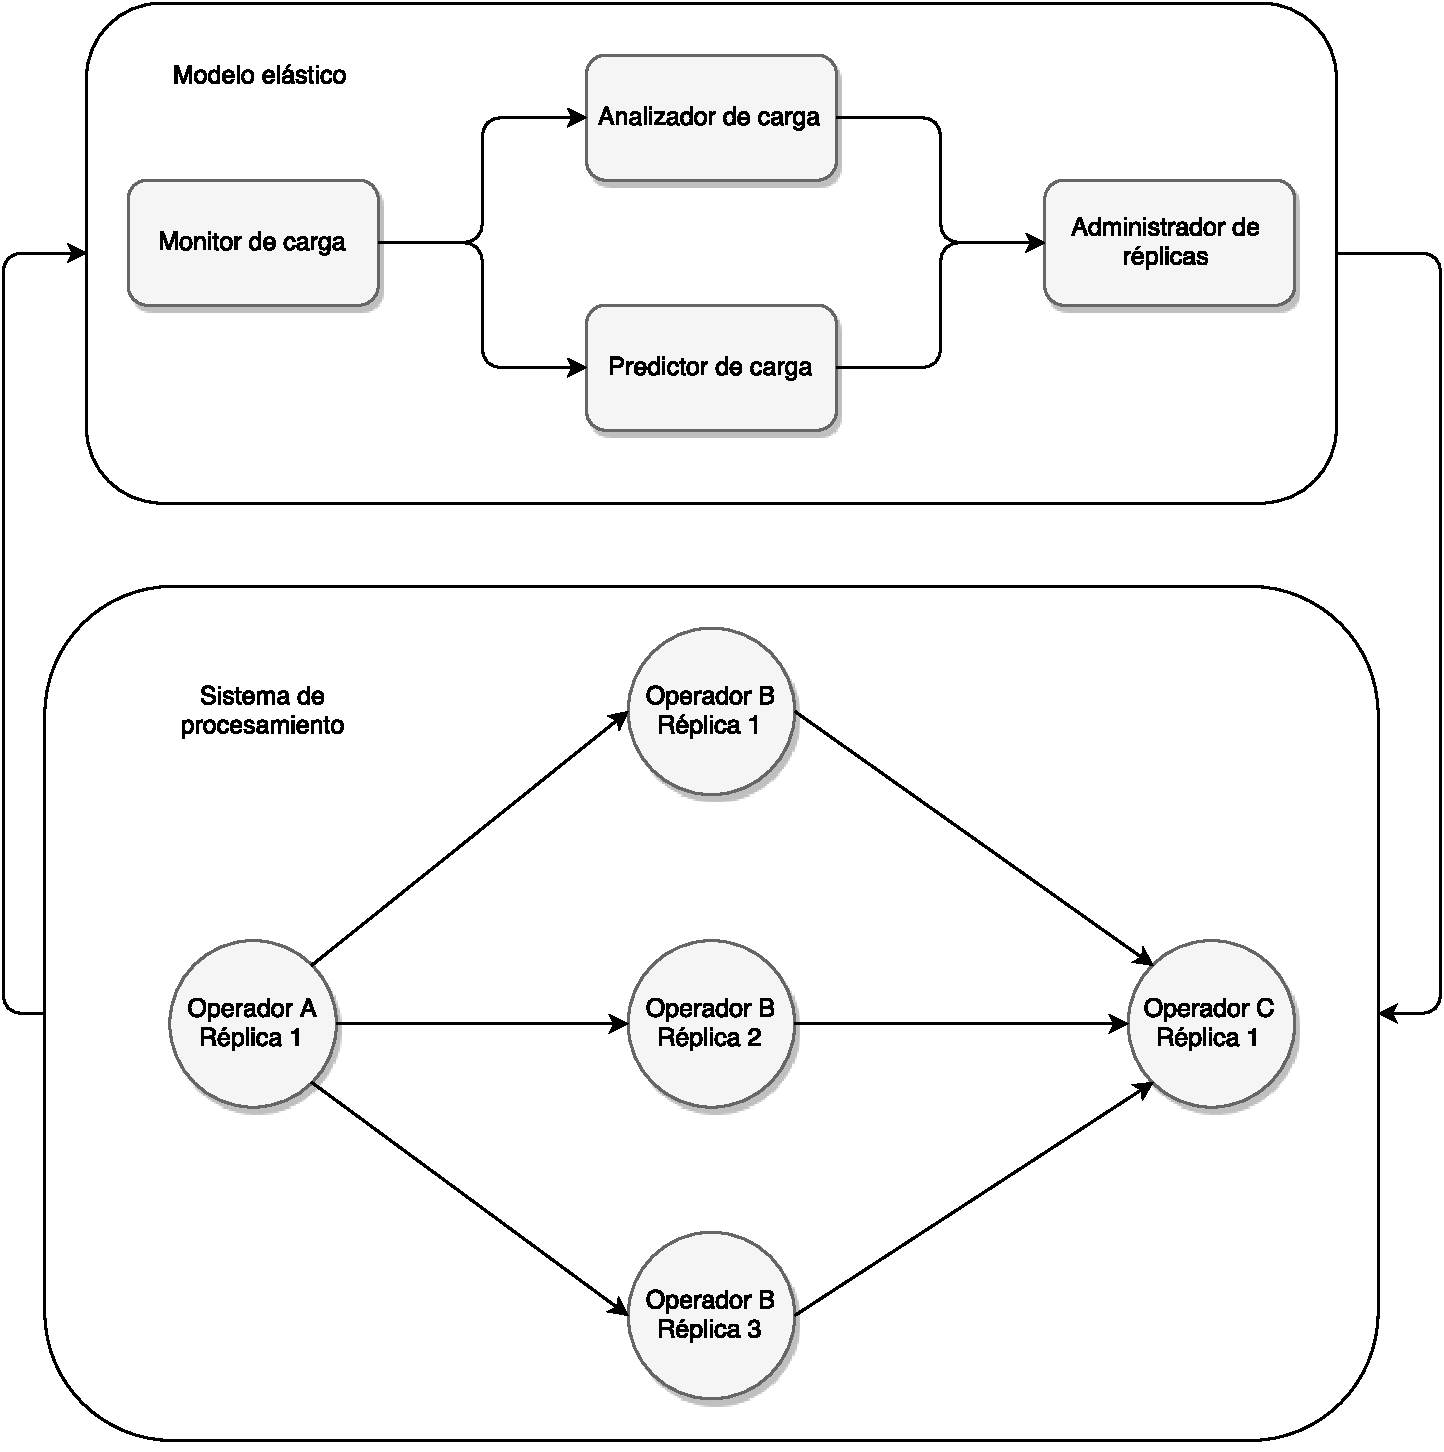
\includegraphics[scale=0.3]{images/Diagrama.pdf}
\end{figure}
\end{frame}

\subsection*{Recolección de los datos}
\begin{frame}{Diseño del modelo elástico}{Recolección de los datos}
El monitor de carga es el encargado de recolectar los datos del grafo de operadores
\begin{itemize}
	\item $\rho = \frac{\lambda}{\mu s}$
	\item Algoritmo reactivo
	\item Algoritmo predictivo $\rightarrow$ Historial
	\begin{itemize}
		\item $n$ muestras
	\end{itemize}
\end{itemize}

\end{frame}

\subsection*{Algoritmo reactivo}
\begin{frame}{Diseño del modelo elástico}{Algoritmo reactivo}
\begin{block}{Analizador de carga}
	Este módulo está enfocado en analizar el comportamiento del operador en el momento
\end{block}

\pause
\begin{alertblock}{}
	\centering
	Umbrales basados en el rendimiento del operador
\end{alertblock}
\end{frame}

\begin{frame}{Diseño del modelo elástico}{Algoritmo reactivo}
\begin{itemize}
\item Análisis del estado del operador $\rightarrow$ Ventana de tiempo $T_r$
\item Tasa de rendimiento $\rho$
\end{itemize}
\hspace{1cm}
\begin{tabular}{c c}
	$\rho > 1$ & Inestable \\
	$1 \geqslant \rho \geqslant 0.5$ & Estable \\
	$\rho < 0.5$ & Ocioso
\end{tabular}

\begin{figure}[ht!]
  \centering
    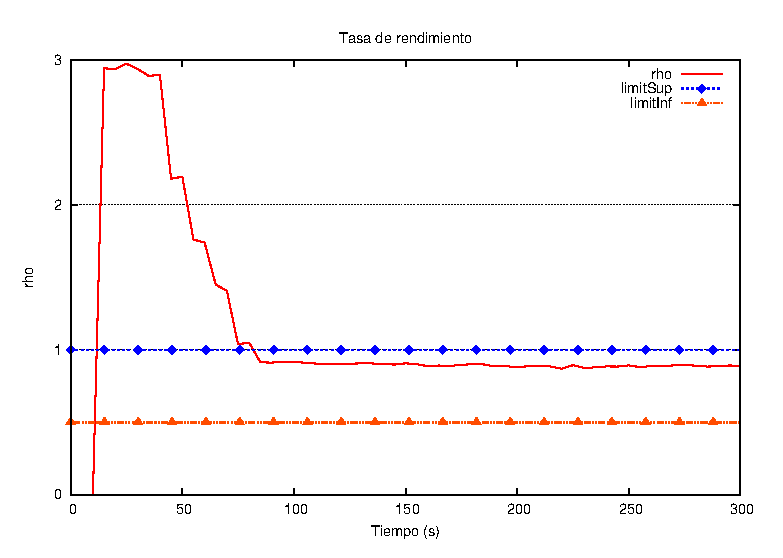
\includegraphics[scale=0.5]{images/Umbrales.eps}
\end{figure}
\end{frame}

\subsection*{Algoritmo predictivo}
\begin{frame}{Diseño del modelo elástico}{Algoritmo predictivo}
\begin{block}{Predictor de carga}
	Este módulo está enfocado en predecir el estado del operador basado en el comportamiento de su historia según las muestras obtenidas por el monitor
\end{block}

\pause
\begin{alertblock}{}
	\centering
	Cadenas de Markov
\end{alertblock}
\end{frame}

\begin{frame}{Diseño del modelo elástico}{Algoritmo predictivo}
\begin{itemize}
	\item Definir muestras en tiempos discretos, las cuales cambian con el tiempo según un proceso estocástico
	\begin{itemize}
		\item Tasa de rendimiento $\rho$
	\end{itemize}
	\item Determinar los estados finitos que se utilizan para la conformación de la cadena
	\begin{itemize}
		\item Ocioso
		\item Estable
		\item Inestable
	\end{itemize}
	\item Obtener una cantidad representativa de muestras para la construcción de la cadena de Markov en el período analizado
	\begin{itemize}
		\item $n$ muestras
	\end{itemize}
\end{itemize}

\end{frame}


\begin{frame}{Diseño del modelo elástico}{Algoritmo predictivo}
\begin{multicols}{2}
\begin{itemize}
	\item Construcción de la matriz de transición
		\begin{itemize}
			\item La transición de estados de un período a otro
		\end{itemize}
\end{itemize}
%\vspace{-5cm}
\begin{center}
\begin{align*}
	P =
	\begin{bmatrix}
		T_{1,1} & T_{1,2} & T_{1,3} \\
		T_{2,1} & T_{2,2} & T_{2,3} \\
		T_{3,1} & T_{3,2} & T_{3,3}
	\end{bmatrix}	
\end{align*}
\end{center}

\vspace*{10cm}

\begin{itemize}
	\item Obtención de la Cadena de Markov
\end{itemize}
\begin{figure}[ht!].
  \centering
    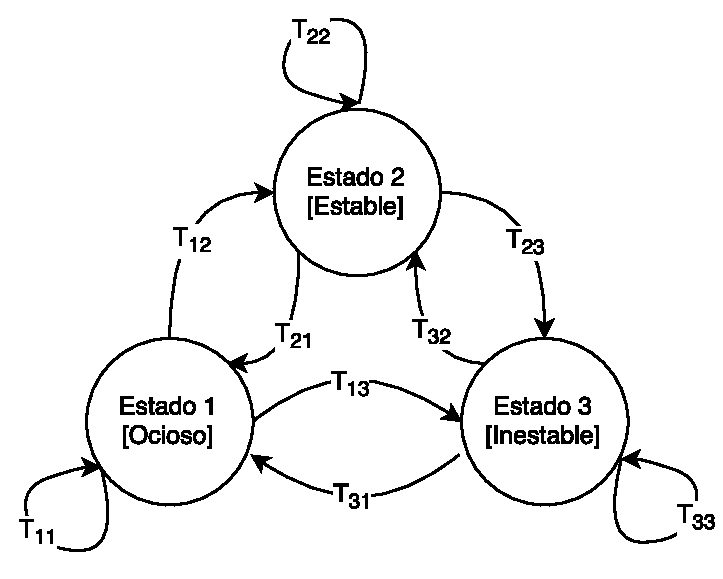
\includegraphics[scale=0.35]{images/CadenaMarkovPredictiva.pdf}
\end{figure}
\end{multicols}
\end{frame}

\begin{frame}{Diseño del modelo elástico}{Algoritmo predictivo}
\begin{itemize}		
	\item Si la cadena es irreducible y sus estados son aperiódicos y positivos recurrentes
	\item Ecuación de Chapman-Kolmogórov $\rightarrow$ Distribución Estacionaria
	\begin{itemize}
		\item La probabilidad que la cadena pueda estar en un estado $i$ en un futuro lejano
	\end{itemize}
\end{itemize}
\vspace{-1cm}
\begin{center}
\begin{align*}
\begin{bmatrix}
	\Pi_1 & \Pi_2 & \Pi_3
\end{bmatrix} _{(t+1)}
\end{align*}
\end{center}
\vspace{-0.5cm}	
\begin{itemize}		
	\item $\sigma(\Pi_1, \Pi_2, \Pi_3) > \alpha$
	\begin{itemize}
		\item No poseer incertidumbre
		\item En caso contrario, no es un comportamiento determinante
	\end{itemize}
\end{itemize}
\end{frame}

\subsection*{Administración del sistema}
\begin{frame}{Diseño del modelo elástico}{Administración del sistema}
\begin{itemize}
\item Administración de la cantidad de réplicas requeridas de cada operador
\item Recursos disponibles de la máquina
\item Según la ventana de tiempo realiza un tipo análisis
\begin{itemize}
	\item $T_r \rightarrow $ Algoritmo reactivo
	\begin{itemize}
		\item $\beta$ alertas consecutivas $\rightarrow$ Modificar la cantidad de réplicas $\omega$
	\end{itemize}
	\item $T_p \rightarrow $ Algoritmo predictivo
	\begin{itemize}
		\item Menor frecuencia
		\item Mayor cómputo
		\item Modifica una mayor cantidad de réplicas $\rightarrow \theta$
	\end{itemize}
\end{itemize}
\end{itemize}
\end{frame}